\documentclass[pre,amsmath,amssymb, twocolumn, showpacs]{revtex4}
\usepackage{dcolumn}
\usepackage{bm}
\usepackage{graphicx}
\usepackage{hyperref}
\usepackage{mathptmx}
\usepackage{subfigure}
\usepackage[utf8]{inputenc}
\usepackage{bbold}
\usepackage{color}
\usepackage{xcolor}
\graphicspath{{Images2/}{../Images2/}}
\newcommand{\RR}{\mathbb{R}}
\newcommand{\ZZ}{\mathbb{Z}}
\newcommand{\Epar}{E_{\|}}
\newcommand{\Eperp}{E_\bot}
\newcommand{\Lpar}{L_{\|}}
\newcommand{\vv}{\mathbf{v}}
\newcommand{\xx}{\mathbf{x}}

\newcommand{\Ata}[1]{{\color{red} #1}}

\makeatletter

\begin{document}


\title{Reporte práctica n: Plantilla }
\author{Autor princial } % (quién tendrá la responsabilidad y por lo tanto una calificación mayor)
\email{ata.kraemer@gmail.com}
\affiliation{Universidad Nacional Autónoma de México, Facultad de Ciencias, México
}
\author{Autor 2}
\affiliation{Universidad Nacional Autónoma de México, Facultad de Ciencias, México
}
\email{ata.kraemer@gmail.com}
 
\date{\today}
\begin{abstract}
 Aquí tienen que escribir un resumen corto de lo que se trata la práctica y su 
 resultado principal. En general rondan las 200 palabras. Aunque pueden ser menos o más. 
\end{abstract}


\maketitle

\section{Introduction}

Aquí tienen que escribir una buena introducción. ¿Por qué es interesante lo que se estudia en esta práctica? Tienen que vender su idea y para eso tienen que citar los trabajos de otro. Fulantino dijo en \cite{art1} que sería interesante tratar el problema. Por otro lado, menganito hace una descripción extensa del problema en \cite{libro1}. 

Alguien mas que trato este problema antes fue perenganito \cite{Internet1}. El sin embargo no resolvio el problema con tales condiciones. Cosa que si se hizo en \cite{Congreso1}. 

Eviten, lo más posible hacer copy-paste, se ve mal y muestra falta de comprensión. Traten de usar sus propias palabras, aunque al final usen una cita. Tampoco caigan en poner ideas que no son suyas sin citar al autor original. Eso es plagio y el castigo es NA en el curso o en caso grave la expulsión de la universidad.  

\subsection{Estado del Arte}

Aquí tienen que dar un resumen de todo lo que se ha hecho y logrado hasta el momento (o tanto como puedan encontrar) sobre el tema. Esto llenará también su bibliografía, lo cual se tomará en cuenta en la calificación. Usen \cite{Internet1, art1, libro1, unpublished1} para citar varias cosas a la vez. Tienen que convencernos que conocen y entienden bien el problema. 

  
\section{Modelo}
\label{model}

En esta sección tendrán que describir el modelo que trataron durante su práctica. Describir con tanto detalle como sea posible. Tiene que poder entender su modelo cualquier persona que tenga un conocimiento mínimo del tema. 

Aquí escribiran las ecuaciones diferenciales a resolverse, y el algoritmo que están usando. 

Para las ecuaciones que se quieren numerar se usa: 

\begin{equation}
\label{eq: maestra}
x = y
\end{equation}

Para las ecuaciones que no se quieren numerar se usa: 

$ x = \frac{z}{w} $

NO TODAS las ecuaciones van numeradas, sólo las importantes. El resto no se numeran. 

Para citar una ecuación, tabla o imagen usan: \ref{eq: maestra}.

\subsection{Variantes}

En general sus prácticas consistirán de varias variantes. Por cada variante tienen que abrir una nueva subsección donde lo expliquen. 

\section{Detalles de la simulación}

Aquí pondrán todos los detalles necesarios para poder reproducir su simulación. Las condiciones iniciales, el número de partículas, la presición de los datos, etc. TODO tiene que estar. 

Si con lo escrito aquí no se puede reproducir los resultados, habrá una penalización fuerte en su calificación. 

\section{Resultados}

Aquí pondrán todas sus gráficas y resultados obtenidos. Es el corazón de su reporte, así que tienen que describir todo cuidadosamente. 

Para poner una imagen usan: 
\begin{figure}
    \centering
    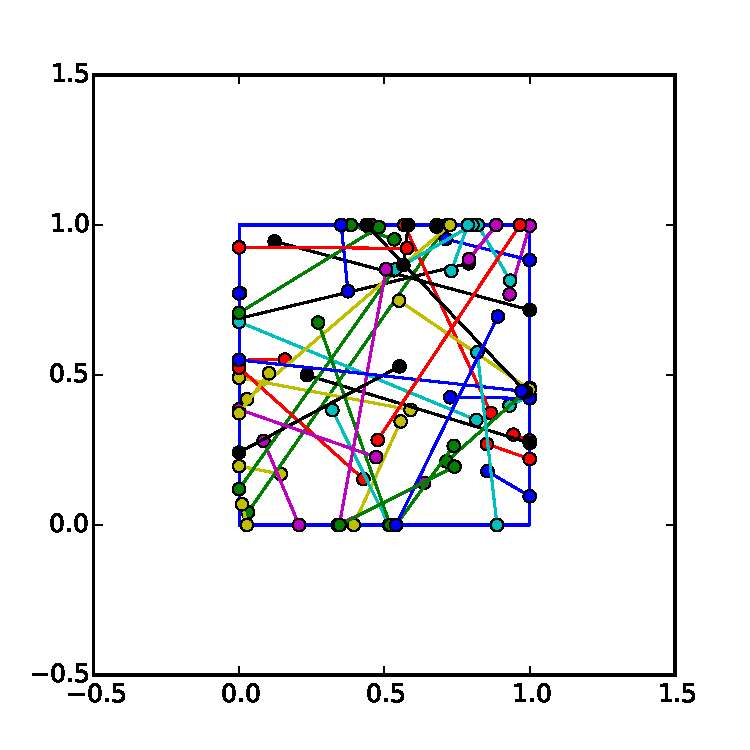
\includegraphics[width=245pt]{fig1.pdf}
    \caption{Aquí va la descripción de la figura. Hagan descripciones completas. Qué significa cada curva. No importa si ya está en el texto. La nota en la figura sirve para facilitar la lectura rápida.}
    \label{fig: figura1}
\end{figure}

\section{Comparación con resultados experimentales y analíticos}

Esta sección es opcional. A veces la comparación puede ir directamente en la sección de resultados, pero a veces la comparación amerita una discusión fuerte por las diferencias que haya entre varios autores, en cuyo caso vale la pena separar la sección. 

\section{Conclusiones}
\label{conclusions}

Casi al final del artículo, tendrán que escribir sus conclusiones. En general la conclusión es del tipo "Lo que se hizo resuelve el problema tal..."; sin embargo, se acepta que lo que hayan desarrollado como modelo no haya funcionado para lo que originalmente querían. En cuyo caso, se menciona eso, pero se da como alternativa para qué sí sirve el modelo. 


\section{Agradecimientos}

Aquí pueden poner a todas las personas que les ayudaron a hacer la práctica. En este curso se acepta que tanto sus colegas como sus amigons les ayuden a entender y a realizar cada paso de las prácticas, a cambio tienen que agradecerles en esta sección.

También agradezcan a cualquiera de los ayudantes si este les brindó asesoría extra (via correo). 

No son necesarios los barbones. De nada les servirá hacer la barba. Simplemente se quiere honestidad. Si pidieron ayuda y les fue dada, agradezcanlo. 

Por último, si están recibiendo alguna beca, marquen la institución que se las da. Es el formalismo que se sigue en las publicaciones y como esto es su entrenamiento a volverse investigadores serios, es bueno que vayan practicando el estilo en las publicaciones, lo cual incluye los agradecimientos a las instituciones. 


\bibliographystyle{apsrev}
\bibliography{Bibliografia} % Esto cargará la bibliografía guardada en el archivo Bibligrafía.bib. 

\end{document}
